% GUIDING QUESTIONS:
%
% What specific problem does your project address, and why is it important?

\begin{frame}{Motivation}
    \huge
    \centering
    Motivation
\end{frame}

\begin{frame}{Aerial Networks}
    \begin{columns}
        \column{0.5\textwidth}
        \begin{itemize}
            \item Flying base stations for 5G/6G applications are popular
                  \cite[12518]{drone-cells}
            \item High line of sight = better transmission, can relay data \cite{lora-drones}
            \item Deployable, dynamic traffic alleviation \cite{drone-cells}

        \end{itemize}

        \column{0.5\textwidth}
        \begin{figure}
            \centering
            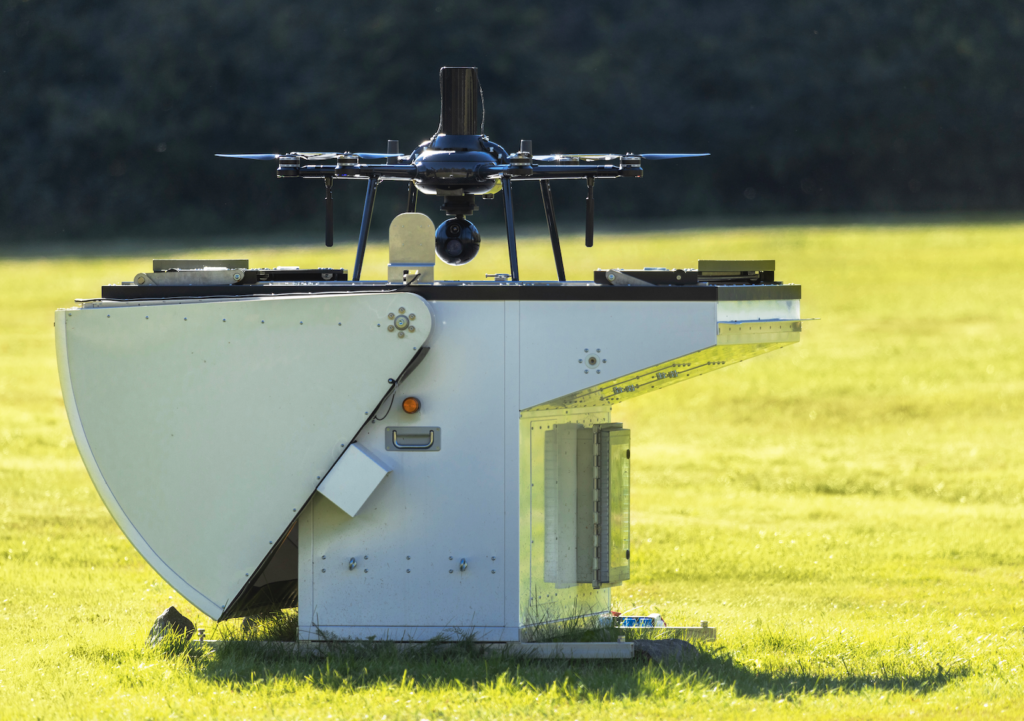
\includegraphics[width=0.75\linewidth]{assets/nokia-drone-network.png}
            \caption{"Drone in a box" from Nokia's 5G drone network platform
                \cite{img:nokia-drone}}
        \end{figure}
    \end{columns}

    % In recent years, mobile aerial networks have been of interest for 5G networking
    % due to the high line-of-sight transmission points available with aerial base
    % stations \cite[12518]{drone-cells}. Aerial networks are composed of multiple
    % aerial robots (often drones \cite[12518]{drone-cells}) which are deployed to
    % relieve traffic loads on existing base stations \cite{drone-cells}, form ad-hoc
    % networks and act as gateways between other networked devices.
    % \cite{lora-drones}

\end{frame}

\begin{frame}{Disaster Relief}

    \begin{columns}
        \column{0.35\textwidth}
        \begin{itemize}
            \item Beyond 5G networking: search \& rescue
            \item Mobile (in motion) networks
            \item Replacement for missing/damaged infrastructure
        \end{itemize}

        \column{0.65\textwidth}
        \begin{figure}
            \centering
            \subfloat[Coastguard flood response in Louisiana \cite{img:coast-guard}]{
                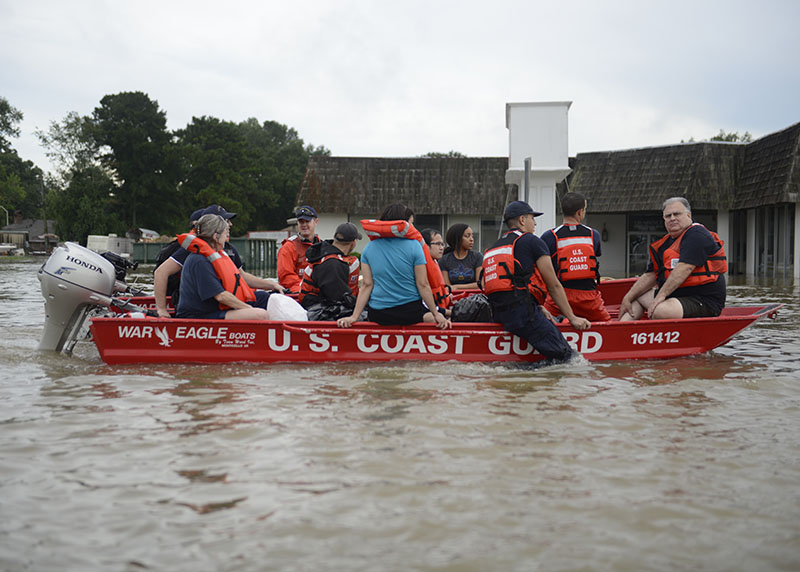
\includegraphics[width=0.4\linewidth]{assets/coastguard.jpeg}
            }
            \subfloat[Flood in Pigeon Hole, Australia \cite{img:rooftop-flood}]{
                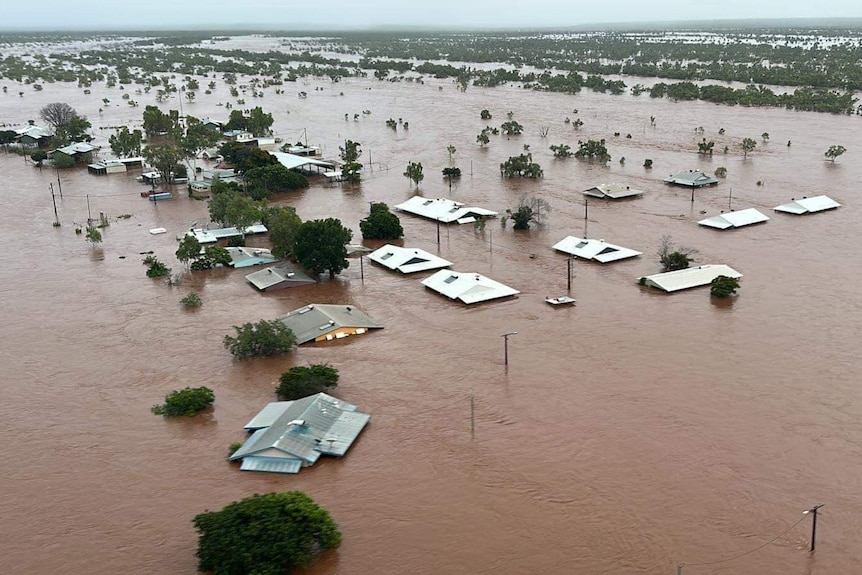
\includegraphics[width=0.4\linewidth]{assets/rooftop-flood.jpg}
            }
            \hspace*{\fill}
            \newline
            \subfloat[Rescue of 4 children in Amazon rainforest \cite{img:operation-hope}]{
                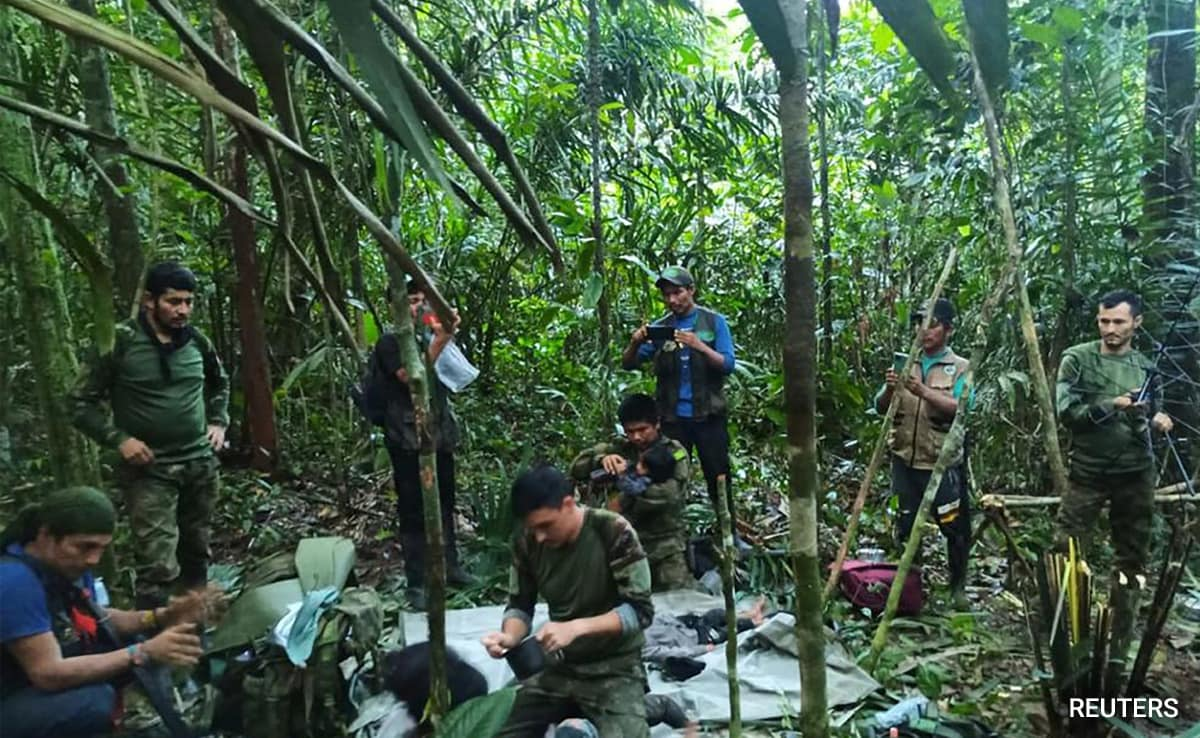
\includegraphics[width=0.4\linewidth]{assets/operation-hope.jpg}
            }
            \hspace*{\fill}
        \end{figure}
    \end{columns}

    % However, aerial networks have additional applications beyond 5G/6G commercial
    % networks. Ad-hoc aerial networks can be used in search-and-rescue or military
    % operations where there is a need for communication links between mobile ground
    % agents during missions.
\end{frame}

\begin{frame}{Application}
    \begin{columns}
        \column{0.5\textwidth}
        \begin{itemize}
            \item Deploy aerial network to connect multiple ground agents
            \item Ground agents move independently
            \item UAVs with radio equipment form ad-hoc network that responds to ground agent
                  movement
        \end{itemize}

        \column{0.5\textwidth}
        \begin{figure}
            \centering
            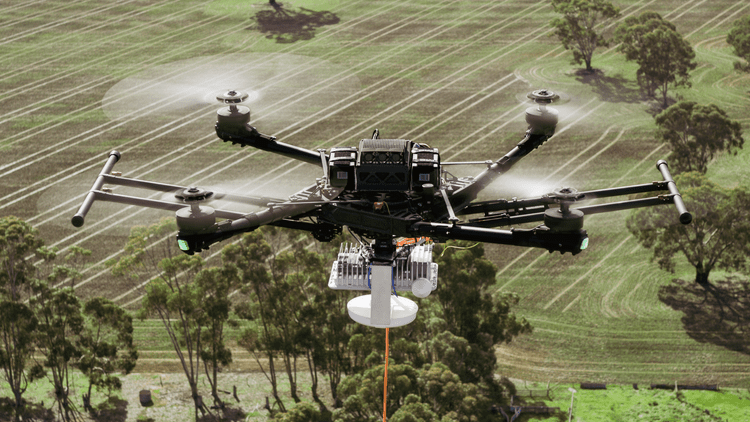
\includegraphics[width=0.75\textwidth]{assets/drone-base-station.png}
            \caption{A commercial drone carrying radio equipment \cite{img:drone-bs}}
        \end{figure}
    \end{columns}
\end{frame}
